\documentclass[tikz]{standalone}

\begin{document}
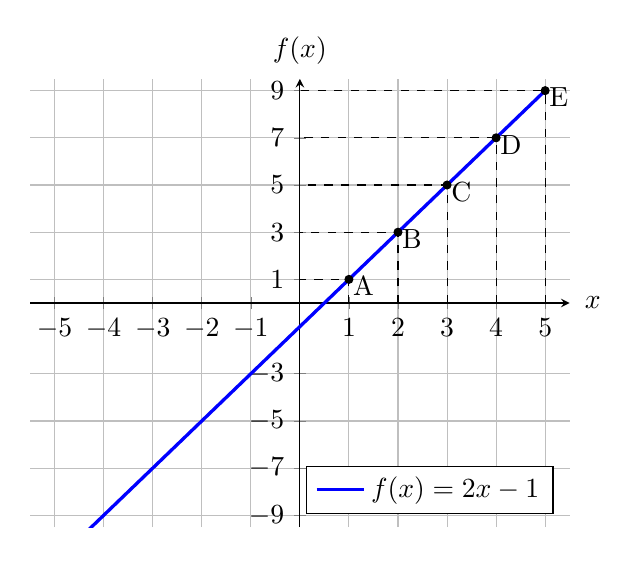
\begin{tikzpicture}
    \begin{axis}[
        xlabel=$x$, ylabel=$f(x)$, legend pos=south east,
        grid=major, xmin=-5.5, xmax=5.5, ymin=-9.5, ymax=9.5,
        axis lines = middle, xtick={-5,-4,-3,-2,-1,0,1,2,3,4,5},
        ytick={-9,-7,-5,-3,0,1,3,5,7,9},
        xlabel style = {at={(axis description cs:1.01,0.5)},anchor=west},
        ylabel style = {at={(axis description cs:0.5,1.01)},anchor=south},
    ]
    \addplot+[blue, very thick, mark=none] plot {2*x-1};
    \addlegendentry{$f(x)=2x-1$}

    \pgfplotsinvokeforeach{1,2,...,5}{% 
        \draw[dashed, thin] (#1,0) |- (0,{2*#1-1});
        \draw[black, fill=black] (#1,{2*#1-1}) circle[radius=0.5mm]
            node[right, xshift=-2pt, yshift=-2.5pt]{%
                \ifnum #1=1 {A}\fi
                \ifnum #1=2 {B}\fi
                \ifnum #1=3 {C}\fi
                \ifnum #1=4 {D}\fi
                \ifnum #1=5 {E}\fi
            };
    }

    \end{axis}
\end{tikzpicture}
\end{document}
